A DSL is defined by three main elements \cite{bib:kleppe}: abstract syntax, concrete syntax and semantics. The abstract syntax defines the main concepts and their relationships, and also include well-formedness rules constraining how the concepts and relationships have to be used. The concrete syntax defines the language notation (textual, graphical or hybrid) and a translational approach is normally used to provide semantics.

Our DSL has been defined in the context of Model-Driven Engineering, thus we used metamodelling techniques \cite{bib:Brambilla} to define the abstract syntax. A metamodel formally describes the structure of the models which are used to represent an aspect of a system at some abstraction level. In our case, we have defined a metamodel to represent the concepts and relationships needed to define governance rules. A model is an instance of a metamodel, and the \emph{conforms to} term is normally used to express this \emph{instance of} relationship between models and metamodels. Thus, models of our language conform to the language abstract syntax metamodel and represent specific instances of governance rules. As concrete syntax, we have opted for a textual language following a typical block-based structure. Thus, each instance of a metaclass is represented by its keyword and a block which contains the name and value of its attributes. Containment references are represented as nested blocks while non-containment references use an identifier to refer the referred element. In the following we will show some examples to illustrate the syntax.

\begin{figure*}[t]
\centering
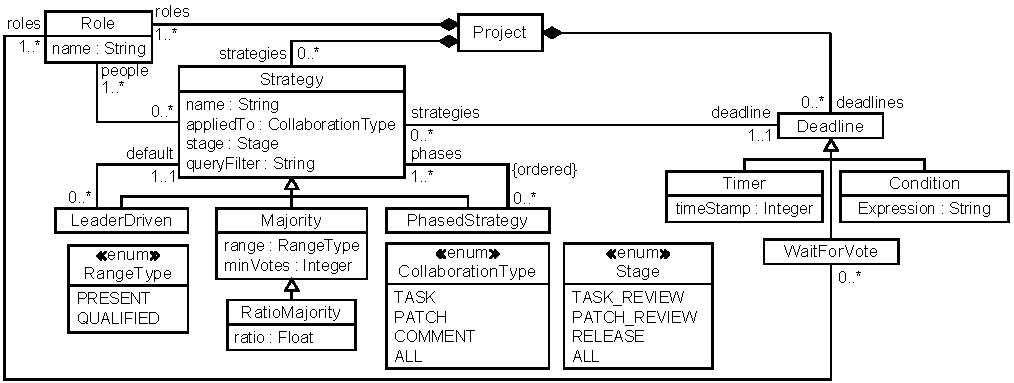
\includegraphics[width=\textwidth]{./figures/decisionStrategy}
\caption{Abstract syntax metamodel of our DSL to represent governance rules (expressed as a UML class diagram).}
\label{fig:decisionStrategy}
\end{figure*}

The abstract syntax metamodel of the language is shown in Figure \ref{fig:decisionStrategy}. The concepts represented in the metamodel covered all the governance aspects identified in our study of OSS projets (Section \ref{sec:motivation}). In particular, a development project (\texttt{Project} metaclass) includes a group of roles of users (\texttt{roles} reference), strategies (\texttt{strategies} reference) and deadlines (\texttt{deadlines} reference). A role has an identifier (\texttt{id} attribute in \texttt{Role} metaclass) and represents a group of people in the development community who can vote. Decision strategies are applied to a particular type of collaborations (\texttt{appliedTo} attribute) according to their nature in the track system (i.e., task, patch or comment) and at a concrete moment (\texttt{stage} attribute) of the process (i.e., task review, patch review, and release). The scope of the strategy can also be defined (\texttt{queryFilter} attribute) (e.g., only those ones which are tagged as high priority). We have defined several decision strategies (included in the hierarchy with root \texttt{Strategy}), which cover the following:

\vspace{0.15em}
\noindent \textbf{Majority Strategy}. This decision strategy (\texttt{Majority} metaclass) accounts for the number of votes received by a collaboration element. Thus, only those elements which have received a support greater than 50\% will be selected. The way of counting votes may differ depending on who is available in the moment of the votation. Since different terminology is used to refer the several types of majority (e.g., \emph{plurality} or \emph{relative majority} used in North America is called \emph{simple majority} in Europe), we will use the neutral term \emph{majority range} to determine exactly how the votes should be counted. Thus, if the range is \texttt{present}, the majority is based on those participants that are present in the moment of voting. Otherwise, a \texttt{qualified} range is based on those participants qualified to vote (presently available or not). A majority strategy can also require a minimum number of votes to be triggered (\texttt{minVotes} attribute). 
    
    As an example, a majority strategy to be applied only to tasks, voted by the committers if they are presently available,  with no need of minimum votes and with a deadline of seven days from the task creation date would be specified as shown in Figure \ref{fig:strategies}a.

\begin{figure*}[t]
\centering
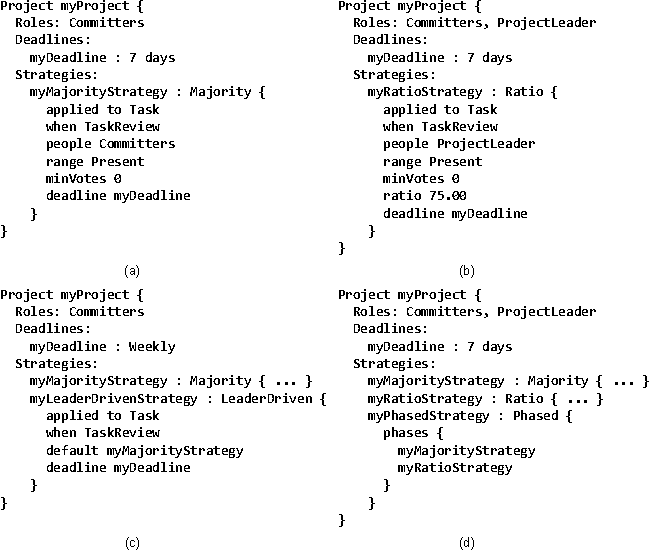
\includegraphics[width=0.8\textwidth]{./figures/strategies}
\caption{Examples of decision strategies: (a) Majority strategy, (b) Majority strategy using ratio (c) Leader-Driven Strategy, (d) Phased Strategy.}
\label{fig:strategies}
\end{figure*}

%{\scriptsize
%\begin{verbatim}
%Project myProject {
%  Roles: Committers
%  Deadlines:
%    myDeadline : 7 days
%  Strategies:
%    myMajorityStrategy : Majority {
%      applied to Task
%      when TaskReview
%      people Committers
%      range Present
%      minVotes 0
%      deadline myDeadline
%    }
%}
%\end{verbatim}
%}

A different percentage for the majority can also be set. In this case the strategy will be called ratio majority (\texttt{RatioMajority} metaclass) and the ratio value must be specified. For instance, this type of strategy would allow implementing well-known majorities such as three-fifths or two-thirds, which may be required for changes on fundamental laws. As example of ratio majority, the definition shown in Figure \ref{fig:strategies}b modifies the strategy presented before to be ratio-based with a ratio of acceptance of 75\% and to be voted only by the project leaders.

%{\scriptsize
%\begin{verbatim}
%Project myProject {
%  Roles: Committers, ProjectLeader
%  Deadlines:
%    myDeadline : 7 days
%  Strategies:
%    myRatioStrategy : Ratio {
%      applied to Task
%      when TaskReview
%      people ProjectLeader
%      range Present
%      minVotes 0
%      ratio 75.00
%      deadline myDeadline
%    }
%}
%\end{verbatim}
%}

\vspace{0.15em}
\noindent \textbf{Leader-Driven Strategy}. When the decision of accepting a collaboration element relies on a user playing the role of leader (e.g., component or project leader), a leader-driven strategy (\texttt{LeaderDriven} metaclass) is followed. Thus, this decision strategy relies on the leader of a collaboration element to decide its acceptance. Next section describes how the leader is represented. The leader must also define a default strategy (\texttt{default} reference) where to delegate the decision in case the leader is not available (i.e. the leader doesn't vote before the deadline)
  
Figure \ref{fig:strategies}c shows an example of leader-driven strategy to be applied only to tasks, with a majority default strategy to be applied when the leader does not make the decision and with a deadline of seven days from the task creation date would be (note that the \texttt{myMajorityStrategy} strategy defined before is reused as default behavior).

%{\scriptsize
%\begin{verbatim}
%Project myProject {
%  Roles: Committers
%  Deadlines:
%    myDeadline : Weekly
%  Strategies:
%    myMajorityStrategy : Majority { ... }
%    myLeaderDrivenStrategy : LeaderDriven {
%      applied to Task
%      when TaskReview
%      default myMajorityStrategy
%      deadline myDeadline
%    }
%}
%\end{verbatim}
%}

\vspace{0.15em}
\noindent  \textbf{Phased Strategy}. This is a composite strategy which allows applying several strategies in a chained way. The strategies are defined and applied in an ordered way (\texttt{phases} reference). Thus, a set of collaboration elements are selected according to the first strategy, the selected ones are then voted again and filtered according to the second strategy, and so on. 

    An example of phased strategy composed of two phases where the first one applies a majority among the committers and with a deadline of seven days from the task creation date, and the second phase, which has a deadline of seven days after the first phase has been done, applies a leader-driven strategy among the project leaders would be (note that \texttt{mymajorityStrategy} and \texttt{myRatioStrategy} are reused) is shown in Figure \ref{fig:strategies}d.

%{\scriptsize
%\begin{verbatim}
%Project myProject {
%  Roles: Committers, ProjectLeader
%  Deadlines:
%    myDeadline : 7 days
%  Strategies:
%    myMajorityStrategy : Majority { ... }
%    myRatioStrategy : Ratio { ... }
%    myPhasedStrategy : Phased {
%      phases {
%        myMajorityStrategy
%        myRatioStrategy 
%      }
%    }
%}
%\end{verbatim}
%}



Regarding the deadlines that trigger a decision strategy, we have currently defined three covering deadlines based on: (1) time (\texttt{Timer} metaclass), (2) a condition to be fulfilled in the collaboration (\texttt{Condition} metaclass) (e.g., the change of a tag in the collaboration model) and (3) a set of users have voted (\texttt{WaitUserVote} metaclass).
 
